\documentclass{article}
\usepackage[margin=1in]{geometry}
\usepackage{graphicx}
\usepackage{pdfpages}
\usepackage{hyperref}
\hypersetup{
    colorlinks=true,
    linkcolor=blue,
    filecolor=magenta,      
    urlcolor=cyan,
}
\usepackage{float}
\usepackage{caption}
\usepackage{subcaption}

\title{CS M152A Lab 2: Clock Design Methodology}
\author{Arnold Pfahnl \\ \small{TA: Mohit Garg, Winter 2021}}
\date{}

\begin{document}
\maketitle
\tableofcontents

\section{Introduction}
In this lab, we take a system clock and output various derived clocks. In general, the groupings of derived clocks in this lab include divide-by-$2^n$ clocks, even division clocks, odd division clocks, and glitchy counter clocks.

In the following sections, nine tasks are explored, with four of these tasks being implemented as submodules of the $clock\_gen$ module. For tasks that are implemented in the $clock\_gen$ module, the overall waveform will be in section \emph{Clock Generator Module}.

\section{Clock Divider by Powers of Two (Task 1)}\label{sec:clk2}
A basic 4-bit counter can represent division-by-2/4/8/16 clocks. To implement this design, I created a 4-bit counter that, given the positive edge of an input clock, resets to $0$ on a reset signal and increments by $1$ otherwise. Bit $0$ (least significant bit) is assigned to the divide-by-2 clock, bit $1$ is assigned to the divide-by-4 clock, bit $2$ is assigned to the divide-by-8 clock, and bit $3$ (most significant bit) is assigned to the divide-by-16 clock. These assignments were made since the least significant bit is a direct division of 2, bit 1 is 4 times as slow, bit 2 is 8 times as slow, and bit 3 is 16 times as slow.

Since these clocks form one of the four deliverable design tasks, their waveforms are under the \nameref{sec:clkgen} section. These clocks are implemented as submodule $clock\_div\_two$ for the $clock\_gen$ module and produce the $clk\_div\_2$, $clk\_div\_4$, $clk\_div\_8$, and $clk\_div\_16$ waveforms.

\section{Even Division Clocks Using Counters}\label{sec:clkeven}
\subsection{Divide-by-32 clock (Task 2)}
In the divide-by-32 clock, the clock flips on every 16th edge of the input clock. In my implementation utilizing a 4-bit counter, if the counter equals $4`b1111$, the clock flips and the counter is reset to $0$.

\begin{figure}[H]
    \centering
    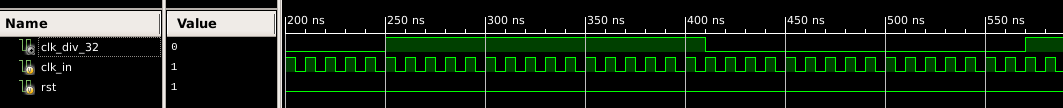
\includegraphics[scale=0.44]{../figs/clock_32.png}
    \caption{$clk\_div\_32$ waveform for a divide-by-32 clock. $clk\_in$ and $rst$ are the input clock and reset, respectively.}
    \label{fig:clk100_200_zoomedout}
\end{figure}

\subsection{Divide-by-28 clock (Task 3)}\label{sec:clk28}
My implementation for the divide-by-28 clock is very similar to the divide-by-32 clock. The only difference is that the clock flips (and counter reset) when the counter equals $4'b1101$.

Since this clock is one of the four deliverable design tasks, the waveform for this clock is under the \nameref{sec:clkgen} section. This clock is implemented as submodule $clock\_div\_twenty\_eight$ for the $clock\_gen$ module and produces the $clk\_div\_28$ waveform.

\section{Odd-Division Clocks Using Counters}
\subsection{33\% duty cycle clocks (Tasks 4-6)}
Basing a clock solely off of when a counter's bits change is not sufficient for odd-division clocks. In this section, 33\% duty cycle clocks are combined to create a 50\% duty cycle divide-by-3 clock.

\textbf{Task 4}: The design first begins with a 33\% duty cycle clock that triggers on the positive edge of the input clock ($odd\_pos$ in the waveform below). To implement this, I used a 2-bit counter that resets to $0$ when the counter reaches $2'd2$ and increments by $1$ otherwise. $odd\_pos$ is set to bit $1$ of the counter. This is because the counter will be in one of three states: $2'b00$, $2'b01$, $2'b10$, and, thus, approximately 33\% of the time bit 1 is set.

\textbf{Task 5}: For the second part of the design, a 33\% duty cycle clock triggers on the negative edge of the input clock ($odd\_neg$ in the waveform below). Since the positive edge clock is already implemented, $odd\_neg$ is implemented such that on the negative input clock edge, $odd\_neg$ is set to the value of $odd\_pos$.

\textbf{Task 6}: Finally, combining the positive- and negative-edge 33\% duty cycle clocks results in a 50\% duty cycle divide-by-3 clock ($odd\_or$ in the waveform below). As the name suggests, this clock is created by OR-ing the positive- and negative-edge 33\% duty cycle clocks together.

\begin{figure}[H]
    \centering
    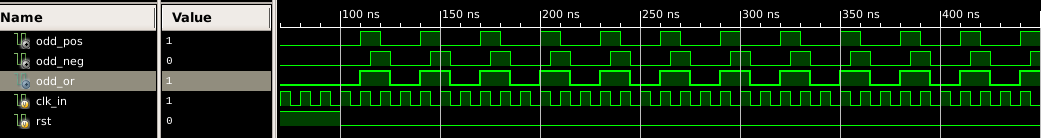
\includegraphics[scale=0.45]{../figs/clock_33_percent.png}
    \caption{$odd\_pos$, $odd\_neg$, and $odd\_or$ waveforms corresponding to a positive-edge 33\% duty cycle clock, negative-edge 33\% duty cycle clock, and a clock composed of the previous two OR-ed together (divide-by-3 clock). $clk\_in$ and $rst$ are the input clock and reset, respectively.}
    \label{fig:clk100_200_zoomedout}
\end{figure}

\subsection{50\% duty cycle divide-by-5 clock (Task 7)}\label{sec:clk5}
Creating a 50\% duty cycle divide-by-5 clock ($clk\_div\_5$), is nearly identical to the steps for creating a 50\% duty cycle divide-by-3 clock in the previous section. Instead of a 2-bit counter, a 3-bit counter is used, and the counter is reset when it reaches $3'd4$.

The positive-edge clock contribution to $clk\_div\_5$ is set to bit 1 of the counter. Since the counter will be in one of five states: $3'b000$, $3'b001$, $3'b010$, $3'b011$, $3'b100$, the clock will be active for 2 of these 5 states, or 2 input cycles out of 5. The clock being active is equivalent to half a cycle, and since we want a divide-by-5 clock, our clock needs to be active for 2.5 input cycles.

The negative-edge clock contributes the extra half cycle. The negative-edge clock is active for the same states, but offset by half of the input clock cycle, providing the additional half cycle when OR-ed with the positive-edge clock.

Since this clock is one of the four deliverable design tasks, the waveform for this clock is under the \nameref{sec:clkgen} section. This clock is implemented as submodule $clock\_div\_five$ for the $clock\_gen$ module and produces the $clk\_div\_5$ waveform.


\section{Pulse/Strobes}
\subsection{Divide-by-100 and divide-by-200 clocks (Task 8)}
To create a divide-by-100 clock with 1\% duty cycle ($clk\_div\_100$ in the waveforms below), I used an 8-bit counter that starts counting from $8'd29$ and resets when it reaches $8'd128$. I specifically chose $8'd128$ since the most significant bit (the eighth bit) will only be set for one input clock cycle. $8'd29$ was chosen as the reset value to make the clock cycle 100 times that of the input clock cycle. As confirmation, the period of one cycle (the difference between the two blue markers of the zoomed-in waveform in Figure~\ref{fig:clk100_200_zoomedin}) is 1000 ns, and since each input clock cycle is 10 ns long, the divide-by-100 clock cycle is, in fact, 100 times longer than the input clock cycle.

Next is the divide-by-200 clock with 50\% duty cycle ($clk\_div\_200$ in the waveforms below). On every positive edge of the input clock, I checked to see if $clk\_div\_100$ was set, and if so the divide-by-200 clock's output flips. In the zoomed-out waveform in Figure~\ref{fig:clk100_200_zoomedout}, we confirm that the cycle length is 2000 ns, or 200 times longer than the input clock cycle.

\noindent \textbf{Zoomed-out view}:

\begin{figure}[H]
    \centering
    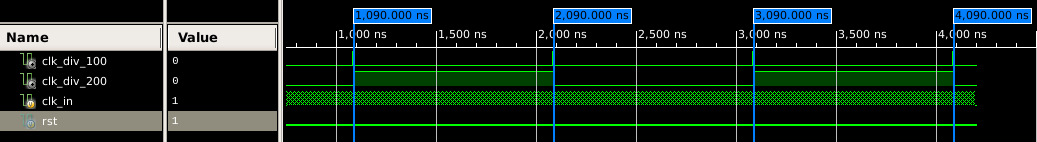
\includegraphics[scale=0.45]{../figs/pulse_1.png}
    \caption{$clk\_div\_100$ and $clk\_div\_200$ zoomed-out waveforms. $clk\_in$ and $rst$ are the input clock and reset, respectively.}
    \label{fig:clk100_200_zoomedout}
\end{figure}


\noindent \textbf{Zoomed-in view}:

\begin{figure}[H]
    \centering
    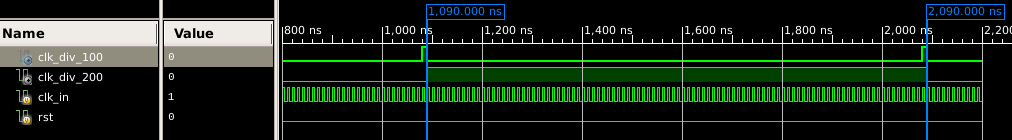
\includegraphics[scale=0.46]{../figs/pulse_2.png}
    \caption{$clk\_div\_100$ and $clk\_div\_200$ zoomed-in waveforms. $clk\_in$ and $rst$ are the input clock and reset, respectively.}
    \label{fig:clk100_200_zoomedin}
\end{figure}

\subsection{Glitchy counter (Task 9)}\label{sec:glitchy}
The glitchy counter ($toggle\_counter[7:0]$) uses a divide-by-4 strobe and input clock to generate an 8-bit counter that increments by 2 on positive edges, and decrements by 5 on every strobe. The following is the beginning of the pattern:

$$0 \rightarrow 2 \rightarrow 4 \rightarrow 6 \rightarrow 1 \rightarrow 3 \cdots$$

I confirmed the output of $toggle\_counter$ to be the same as the expected pattern by viewing the waveform of $toggle\_counter$ in Figure~\ref{fig:clkgen}.

Since this clock is one of the four deliverable design tasks, the waveform for this clock is under the \nameref{sec:clkgen} section. This clock is implemented as submodule $clock\_strobe$ for the $clock\_gen$ module and produces the $toggle\_counter[7:0]$ waveform.

\section{Clock Generator Module}\label{sec:clkgen}
The clock generator module, $clock\_gen$, implements four clock submodules producing a total of seven clock signals from one input clock signal $clk\_in$ and one reset signal $rst$. 

The specific clocks produced are a divide-by-2 clock $clk\_div\_2$, a divide-by-4 clock $clk\_div\_4$, a divide-by-8 clock $clk\_div\_8$, and a divide-by-16 clock $clk\_div\_16$ all from the \nameref{sec:clk2} section and produced by the $clock\_div\_two$ submodule, a divide-by-28 clock $clk\_div\_28$ from the \nameref{sec:clk28} section produced by the $clock\_div\_twenty\_eight$ submodule, a divide-by-5 clock $clk\_div\_5$ from the \nameref{sec:clk5} section produced by the $clock\_div\_five$ submodule, and a glitchy counter $toggle\_counter[7:0]$ from the \nameref{sec:glitchy} section produced by the $clock\_strobe$ submodule. 

Figure \ref{fig:clkgen} contains the waveforms produced by the $clock\_gen$ module clocks, and Figure \ref{fig:schem} contains a high-level schematic of the $clock\_gen$ module, its submodules, and its input and output ports.

\subsection{Simulation Waveforms}
Figure~\ref{fig:clkgen} contains the waveforms for the clocks generated by the $clock\_gen$ module. Figure \ref{fig:clkgen2}, specifically provides a zoomed-out view that allows for a better look at longer waveform cycles such as $clk\_div\_28$ and $clk\_div\_16$.

\begin{figure}[H]
    \centering
    \begin{subfigure}{\textwidth}
        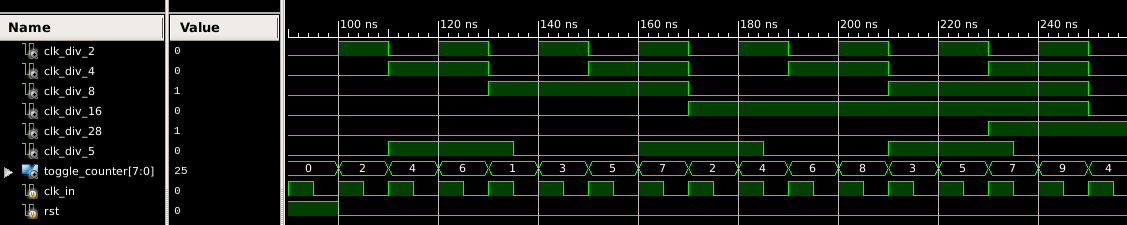
\includegraphics[scale=0.41]{../figs/clock_gen.png}
        \caption{$clock\_gen$ waveforms zoomed in.}
        \label{fig:clkgen1}
    \end{subfigure}
    \begin{subfigure}{\textwidth}
        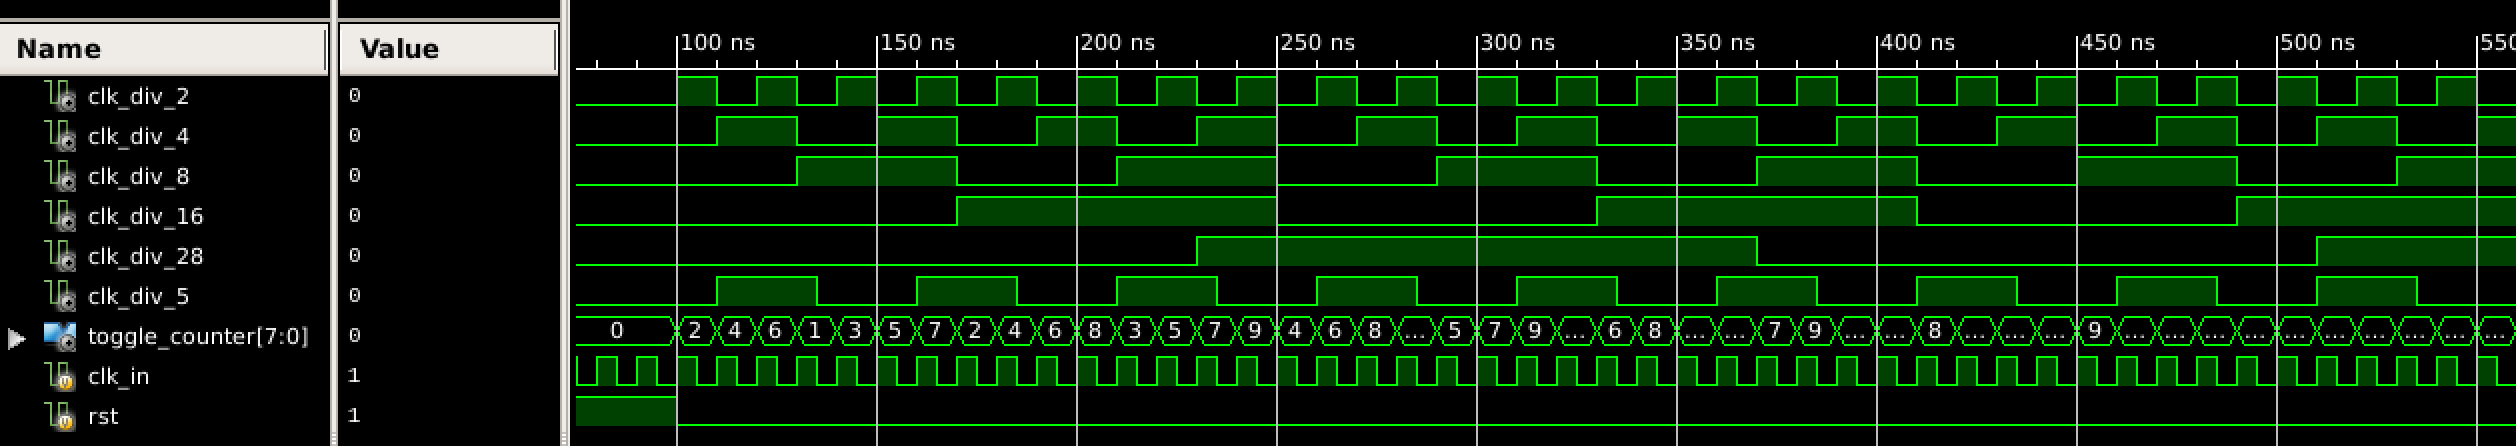
\includegraphics[scale=0.37]{../figs/clock_gen_zoom_out.png}
        \caption{$clock\_gen$ waveforms zoomed out.}
        \label{fig:clkgen2}
    \end{subfigure}
    \caption{$clock\_gen$ waveforms.}
    \label{fig:clkgen}
\end{figure}


\noindent From top to bottom:
\begin{enumerate}
    \item Divide-by-2 clock $clk\_div\_2$ from section \ref{sec:clk2}
    \item Divide-by-4 clock $clk\_div\_4$ from section \ref{sec:clk2}
    \item Divide-by-8 clock $clk\_div\_8$ from section \ref{sec:clk2}
    \item Divide-by-16 clock $clk\_div\_16$ from section \ref{sec:clk2}
    \item Divide-by-28 clock $clk\_div\_28$ from section \ref{sec:clk28}
    \item Divide-by-5 clock $clk\_div\_5$ from section \ref{sec:clk5}
    \item Glitchy counter $toggle\_counter[7:0]$ from section \ref{sec:glitchy}
    \item Input 100 MHz clock $clk\_in$
    \item Reset signal $rst$
\end{enumerate}

\subsection{Clock Generator Module Schematic}
The module schematic is depicted in Figure \ref{fig:schem}. All submodules share the same input clock and input reset signal.
\begin{figure}[H]
    \centering
    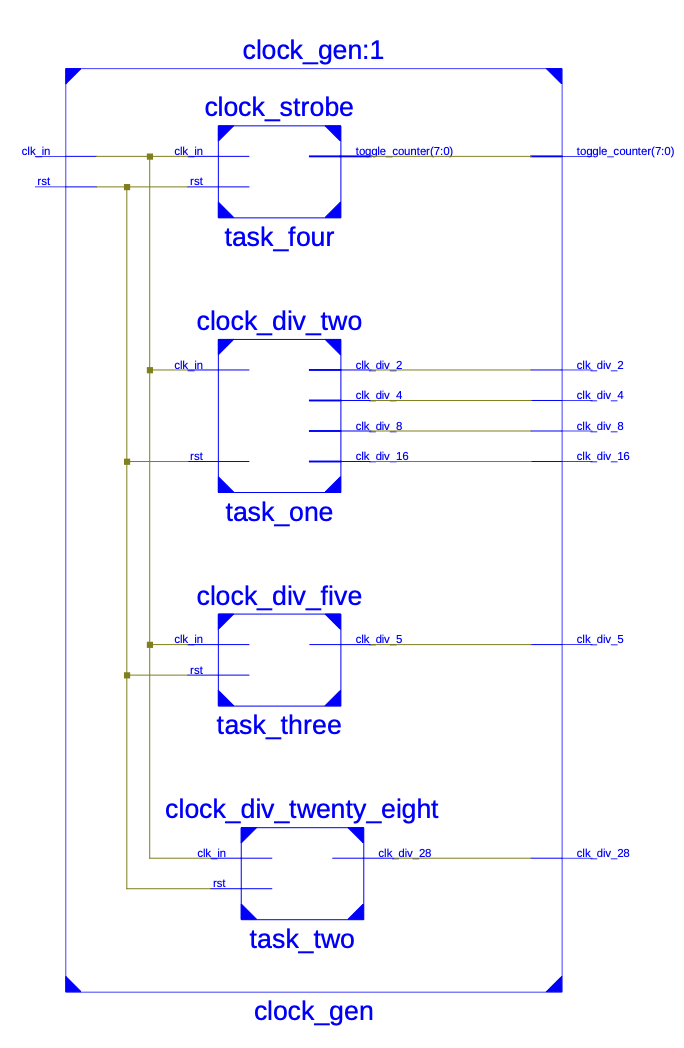
\includegraphics[scale=0.6]{../figs/schematic.png}
    \caption{$clock\_gen$ schematic.}
    \label{fig:schem}
\end{figure}

\subsection{ISE Design Summary}
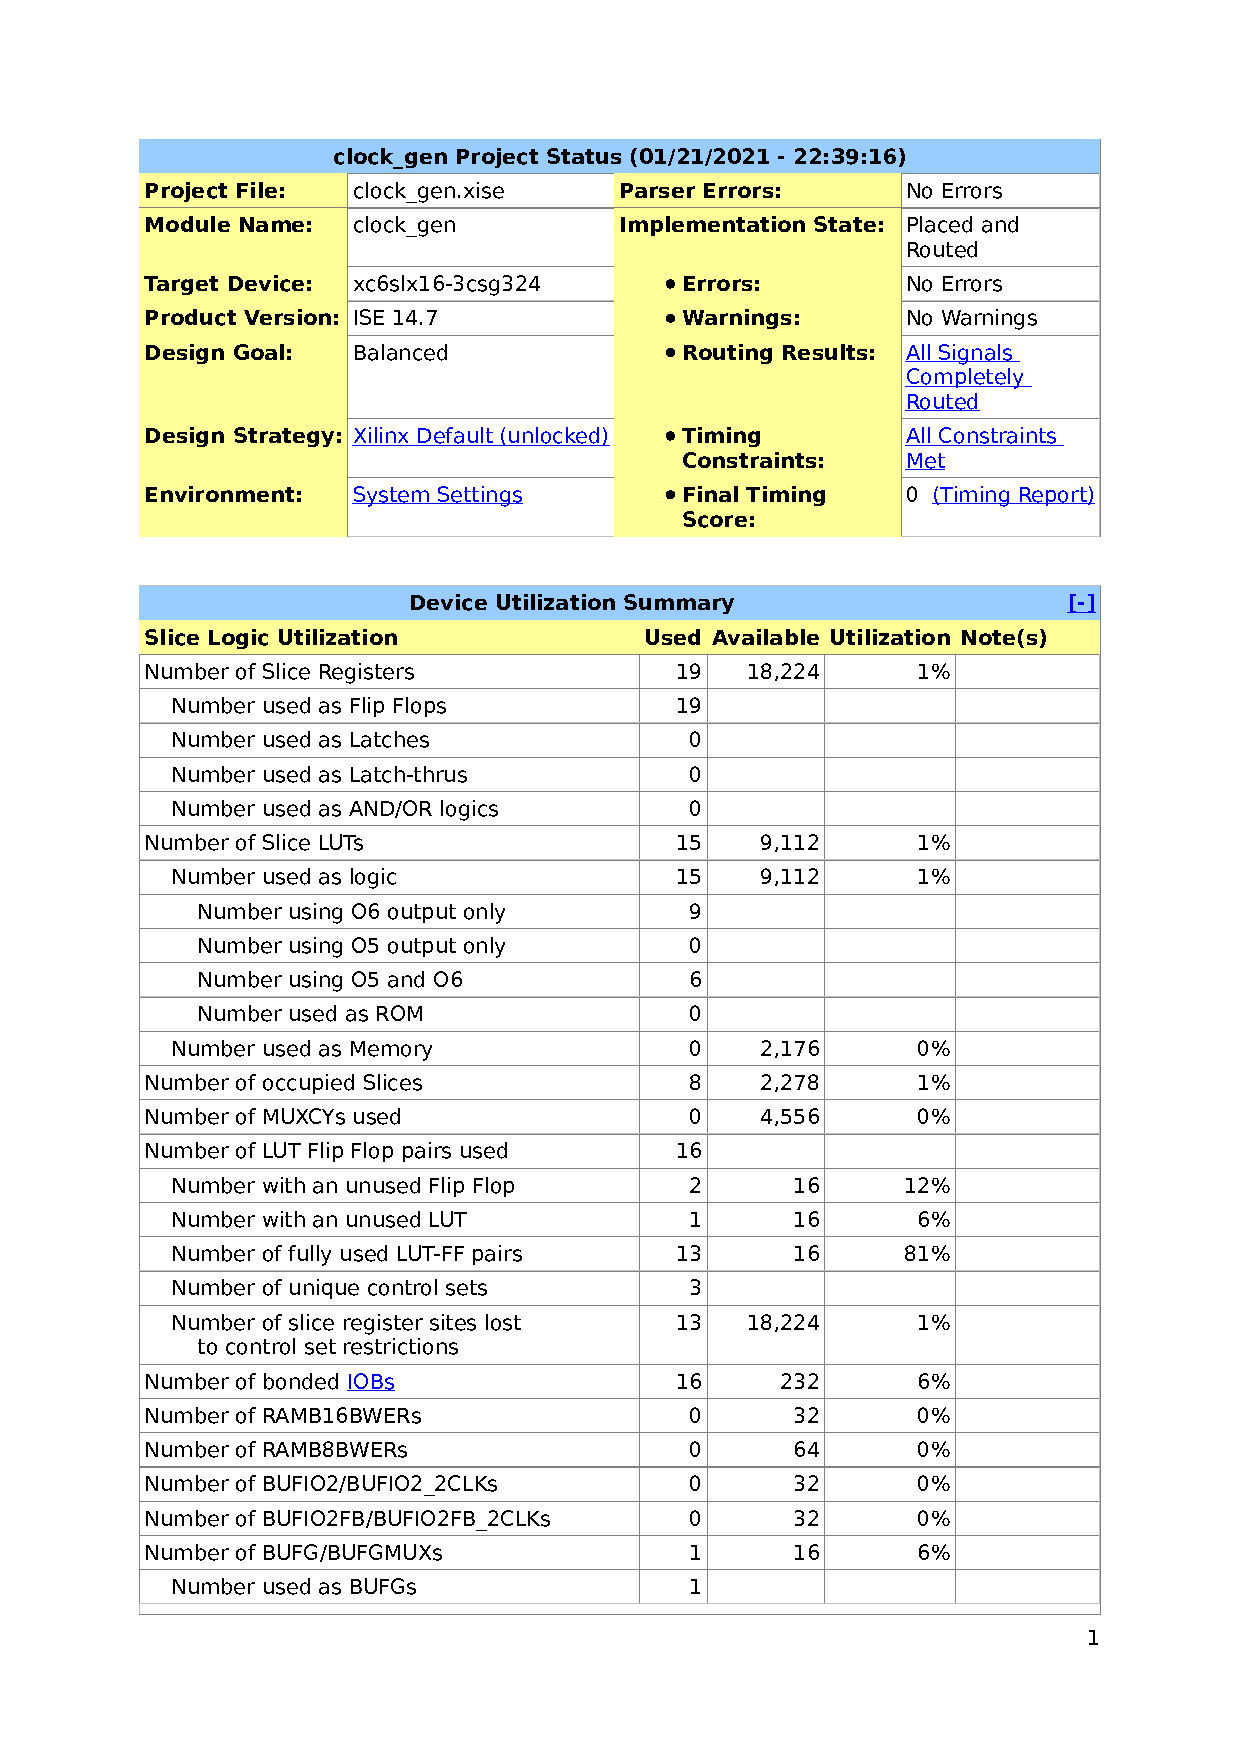
\includepdf[pages=-]{../clock_gen/print.pdf}
\section{Conclusion}
In this lab I was able to successfully implement divide-by-$2^n$ clocks, even division clocks, odd-division clocks, pulses, strobes, and a glitchy counter.

The biggest difficulty I had with this lab was understanding the odd-division clocks. However, after doing my own research on the subject, and drawing out the clock signals by hand, I was able to understand how and why they worked, as well as how to implement them.

Overall, this lab was a great introduction to clocking and implementing sequential circuits. I don't have any suggestions for improvement at this time.
\end{document}